\chapter{Numerické simulace hvězdného větru}

V předcházející kapitole jsme se stručně seznámili se způsobem, kterým lze úspěšně parciální diferenciální rovnice převést na řešitelný numerický problém. Studovali jsme je na jednotlivých zjednodušených typech parciálních diferenciálních rovnic, které však již v některých aspektech odráželi vlastnosti hydrodynamických rovnic. Nyní jsme vlastně již jen krůček od sestavení vlastního hydrodynamického kódu, který budeme moci použít pro studium praktického astrofyzikálního problému. V~této kapitole probereme základní pojmy, veličiny a rovnice z~klasické hydrodynamiky potřebné k~sestavení rovnic popisujících hvězdný vítr. Zvolená symetrie popisu koresponduje s~předpokládanou symetrií hvězdného větru. Pochopení matematického popisu hydrodynamiky je nezbytným krokem při sestavování vlastního kódu. V~další části této kapitoly se pak již zaměříme na numerické řešení těchto rovnic, metodu výpočtu a další aspekty, které je nutné znát pro tvorbu kódu. Na závěr si sestavíme co nejjednoduší hydrodynamický kód, který použijeme pro simulaci dvou nejznámějších typů hvězdného větru, slunečního a zářením hnaného větru horkých hvězd.
\section{Základní rovnice hydrodynamiky}
K~popisu pohybu kontinua můžeme použít dva alternativní přístupy, Eulerův popis a Langrangeův popis. V~Eulerově popisu je pohyb popsán vůči pevnému souřadnicovému systému (ne nutně inerciálnímu). Hydrodynamické rovnice jsou potom parciální diferenciální rovnice vzhledem k~prostoru a času, popisující vývoj jednotlivých hydrodynamických veličin. Naproti tomu v~Lagrangeově popisu je celé kontinuum rozděleno na určité elementární části objemu a je sledován pohyb každé této elementární části. Oba dva tyto přístupy mají své výhody a nevýhody. V~našem popisu a kódu se omezíme na první, tedy Eulerův přístup.

Nejprve zavedeme značení jednotlivých hydrodynamických veličin, kterého se budeme držet v~celém dalším textu. Základními hydrodynamickými veličinami jsou skalární hustota $\rho$, tlak $p$, vektorová rychlost elementu kontinua $\vec{v}$ a vnitřní energie plynu $U$. Tyto veličiny jsou vzájemně svázány pomocí hydrodynamických rovnic. Dále se v~našem přístupu omezíme na ideální tekutinu, nebudeme tedy započítávat vazkost tekutiny. To je v~případě drtivé většiny astrofyzikálních aplikací zcela oprávněná aproximace. V~takovém případě lze kontiunum popsat Eulerovými rovnicemi: rovnicí kontinuity, rovnicí pro hybnost a rovnicí pro energii. Obecný tvar rovnice kontinuity je podle {\citep{Landau}}
\begin{eqnarray}
		\frac{\partial{\rho}}{\partial{t}}+{\rm div}({\, \rho \vec v})=0.
		\label{konti}
\end{eqnarray} 
Obecný tvar rovnice pro hybnost za předpokladu gravitačního zrychlení $\vec{g}_*$ a 
zářivého zrychlení $\vec{g}_{\rm rad}$, lze psát 
\begin{eqnarray}
	\label{hybnost}
	\frac{\partial \vec{v}}{\partial{t}}+(\vec{v}.\nabla )\vec{v}
		+\frac{\nabla p}{\rho} = \vec{g}_*+\vec{g}_{\rm rad}.
\end{eqnarray}
Obecný tvar rovnice pro energii je dán
	\begin{eqnarray}
	\label{energie}
		\frac{\partial }{\partial{t}}\left(\frac{1}{2}v^2+\rho U\right)-{\rm div}\left(\rho\vec{v}(\frac{1}{2}v^2+H)\right)=0,
	\end{eqnarray}
kde $U$ značí vnitřní energii plynu a $H$ entalpii. V~rámci naší problematiky rovnici pro energii nebudeme nadále uvažovat. Pro jednoduchost budeme uvažovat pouze izotermické procesy (pokud bychom však chtěli započítat realističtější neizotermické procesy, je  níže uvedený postup analogický). V~rámci této aproximace ještě doplníme soustavu o~stavovou rovnici ideálního plynu
\begin{equation}
\label{staveq}
p=a^2\rho,
\end{equation}
kde $a$ značí rychlost zvuku a v~případě ideálního plynu závisí na teplotě podle vztahu
\begin{equation}
\label{soundspeed} 
a=\sqrt{\frac{k_B T}{\mu m_H}}.
\end{equation}
$k_B=1.3807\, .10^{-16}$[erg K$^{-1}$] je Boltzmannova konstanta, $m_{H}$ je hmotnost atomu vodíku a $\mu_{m}$ je střední molekulová hmotnost plynu. Přesný výpočet $\mu$ je poměrně komplikovaný a závisí na určení stupně ionizace všech chemických elementů v~plynu.
\section{Základy numerické dynamiky tekutin}
\subsection{Konzervativní schéma}
Hydrodynamické rovnice lze numericky formulovat jak v Langrangeově formalismu, tak v Eulerově formalismu. Základní vlastností Lagrangeova přístupu je, že celková hmota se zachovává. Pro numerické schéma v Eulerově formalismu to nemusí být obecně pravda. Je však možne Eulerovy rovnice do konzervativní formy přepsat. Jaký je tedy v tom rozdíl ? Uvažme derivaci z rovnice kontinuity
\begin{equation}
\label{conserve_example}
\frac{\partial \rho u}{\partial x},
\end{equation}
kterou diskretizujeme následujícím způsobem,
\begin{equation}
\label{con_1}
\frac{\partial \rho u}{\partial x}=\frac{(\rho u)_{i}-(\rho u)_{i-1}}{\Delta x}.
\end{equation}
Můžeme však také derivaci (\ref{conserve_example}) rozepsat
\begin{equation}
\rho \frac{\partial u}{\partial x}+u\frac{\partial \rho}{\partial x}.
\end{equation}
Což s použitím stejné numerické aproximace jako v případě (\ref{con_1}) vede
\begin{equation}
\label{con_2}
\rho \frac{\partial u}{\partial x}+u\frac{\partial \rho}{\partial x} = \rho_i\frac{u_i-u_{i-1}}{\Delta x}+u_i\frac{\rho_i-\rho_{i-1}}{\Delta x},
\end{equation}
Vidíme, že výsledne numerické schéma (\ref{con_1}) a (\ref{con_2}) aproximované derivace (\ref{conserve_example}) není stejné, ač vychází ze stejné 
rovnice a stejného numerického přístupu. Ale zachovává vztah (\ref{con_1}) skutečně hmotu na rozdíl od (\ref{con_2})? Abychom se o tom přesvědčili, stačí 
sečíst výsledný vztah přes všechny body sítě.  Zvolme pro jednoduchost případ sítě se čtyřmi body, dostáváme
\begin{equation}
\label{conserve_form_expl_1}
\frac{(\rho u)_{1}-(\rho u)_{0}}{\Delta x}+\frac{(\rho u)_{2}-(\rho u)_{1}}{\Delta x}+\frac{(\rho u)_{3}-(\rho u)_{2}}{\Delta x}
\end{equation}
ze kterého je ihned patrné, že zbývají pouze členy na okraji $i=0$ a $i=3$, tedy pouze na tom kolik hmoty vchází dovnitř a kolik vychází ven. V případě
druhém (\ref{con_2}) je situace komplikovanější
\begin{equation}
\label{conserve_form_expl_2}
\rho_1\frac{u_1-u_{0}}{\Delta x}+u_1\frac{\rho_1-\rho_{0}}{\Delta x}+\rho_2\frac{u_2-u_{1}}{\Delta x}+u_2\frac{\rho_2-\rho_{1}}{\Delta x}+\rho_3\frac{u_3-u_{2}}{\Delta x}+u_3\frac{\rho_3-\rho_{2}}{\Delta x}
\end{equation}
jednotlivé vnitřní členy se nevyruší, pokud přidáme další bod sítě přidáme i další člen a výsledná suma je větší. Nelze tedy hovořit o zachování hmoty.

V praxi je použití konzervativního schématu velkou výhodou, poněvadž respektuje fyzikální podstatu problému. Navíc oproti nekonzervativním schématům vykazují větší stabilitu a přesnost v případě existence rázových vln během studovaného procesu. Eulerovy hydrodynamické rovnice (rovnici pro energii pro jednoduchost neuvažujeme) tedy přepíšeme do konzervativního tvaru
\begin{equation}
\label{euler_conserve}
\vec{u}_t+\vec{F}(\vec{u})_{x} = 0.
\end{equation}
kde
\begin{equation}
\label{vector_form}
\vec{u} = \begin{pmatrix}
		\rho \\
		\rho v
		\end{pmatrix}\quad,\quad\vec{F}(\vec{u}) = \begin{pmatrix}
						\rho v \\
						\rho v^2 + p
					\end{pmatrix}.
\end{equation}
Abychom lépe ilustrovali výhody, které přináší tento přístup, zavedeme speciální typ sítě, který se ve spojitosti s konzervativním typem schématu často používá. Jedná se o střídavou síť ( v anglické literatuře označovanou jako {\it staggered}), ve které hustota (a další skalární veličiny) je definována ve středu výpočetní buňky, zatímco rychlost (vektorová veličina) na jejím okraji (viz. obrazek \ref{figure:grid_staggered}). S použitím konzervativního schématu Eulerových rovnic, lze pak říci, že hustota ve středu výpočetní buňky je dána tokem hmoty, přes její okraje.
\subsection{Technika oddělených toků}
\label{technikaodd}
Tato metoda, známá spíše pod svým anglickým názvem {\it flux splitting} technika \citep[stránka 415]{Hirsch2002}, umožňuje rozdělit řešení parciální diferenciální rovnice na části, kde každá část reprezentuje jeden samostatný člen z~uvažované rovnice. Schématicky zapsáno, pro dynamický systém daný rovnicí
\begin{equation}
\frac{\partial \vec{u}}{\partial t}=\mathcal{L}(\vec{u})
\label{schemasplit}
\end  {equation}
je $\vec{u}$  je reprezentováno sloupcovým vektorem (\ref{vector_form}). Operátor $\mathcal{L}(\vec{y})$ můžeme rozložit na součet částečných operátorů $\mathcal{L}(\vec{u})=\mathcal{L}_1(\vec{u})+\mathcal{L}_2(\vec{u})+\dots +\mathcal{L}_m(\vec{u})$, přičemž každý operátor představuje jeden člen z rovnice. Tedy například advekční člen, člen odpovídající tlakovým, gravitačním silám apod. Numerické řešení rovnice \eqref{schemasplit} pak obdržíme postupnou aplikací jednotlivých operátorů 
\begin{eqnarray}
\vec{u}^{n+1/m} &=&\mathcal{L}_1(\vec{u}^n,\Delta{t}), \\
\nonumber \vec{u}^{n+2/m} &=&\mathcal{L}_2(\vec{u}^{n+1/m},\Delta{t}), \\
\nonumber \vec{u}^{n+3/m} &=&\mathcal{L}_3(\vec{u}^{n+2/m},\Delta{t}), \\
\nonumber \vdots &=&\vdots, \\
\nonumber \vec{u}^{n+1} &=&\mathcal{L}_m(\vec{u}^{n+m-1/m},\Delta{t})
\end{eqnarray}

\section{Advekční člen}
Rozepíšeme Eulerovy rovnice 1D v kartézských souřadnicích a v konzervativním tvaru ({\ref{euler_conserve}) dostáváme
\begin{eqnarray}
\label{euler_expanded}
\frac{\partial{\rho}}{\partial t} + \frac{\partial{\rho v}}{\partial x} = 0 \\
\frac{\partial{\rho v}}{\partial t} + \frac{\partial{\rho v^2}}{\partial x}+\frac{\partial p}{\partial x} = 0
\end{eqnarray}
první dva členy v obou rovnicích reprezentují změnu hustoty a momentu hybnosti jako výsledek přenosu hmoty a memonetu hybnosti podél sítě. To je podstata advekčního členu, nedochází k celkové změně hmotnosti a momentu hybnosti, vyjma toho co do systému vchází a odchází v důsledku okrajových podmínek. Z numerického hlediska je však podstatné, aby ta část numerického výpočtu, která počítá advekční člen byla provedena konzistentně. Tím máme na mysli, aby advekce všech fyzikálních veličin, tedy jak hustoty, tak momentu hybnosti byly počítány stejným způsobem. Jinak řečeno, pokud dochází k přetoku hmotnostního elementu z jedné výpočetní buňky do druhé, dochází také ve stejný okamžik k přetoku momentu hybnosti. 
\begin{figure}
\centering
\scalebox{0.85}{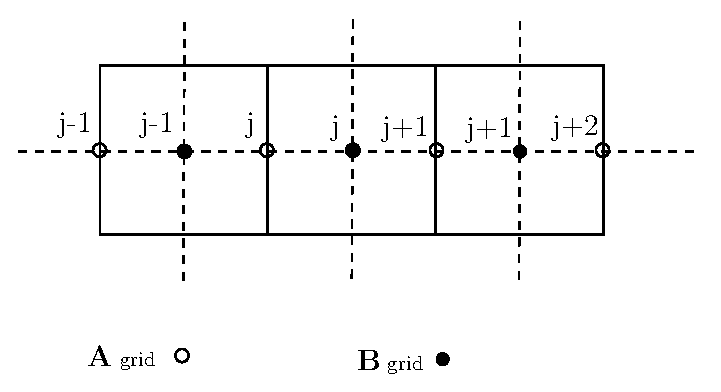
\includegraphics{grid.eps}}
\caption{\it Střídavý typ sítě, skalární veličiny jsou definováne na středu výpočetní buňky - body {\bf B}, vektorové veličiny jsou definovány na okrajích výpočetní buňky - body {\bf A}.}
\label{figure:grid_staggered}
\end{figure}
Pro ilustraci se podívejme na rovnici kontinutiy (\ref{euler_expanded}), obecné numerické schéma pro řešení této rovnice pro advekci
\begin{equation}
\rho_{B,i}^{n+1} = \rho_{B,i}^{n} - \frac{\Delta t^{n+1/2}}{\Delta x_{B,i}}(F_{i+1}-F_i) = \rho_{B,i}^n-\frac{\Delta t^{n+1/2}}{\Delta x_{B,i}^{n}}\left((\overline{\rho} v)_{i+1}-({\overline \rho} v )_{i}\right)
\end{equation}
kde 
\begin{equation}
\Delta x_{B,i} = x_{A,i+1}-x_{A,i}.
\end{equation}
Pro vysvětlenou: horní index u časového kroku je zde proto, že velikost časového kroku se během časového vývoje mění tak, aby vždy byla splněna Courantova podmínka stability. Hustota $\overline{\rho}$ vystupující v členech odpovídající toku hmoty skrze hranice výpočetní buňky, by měla co nejvíce odpovídat množství hmoty protékající skrze hranice buňky. Její hodnotu dostaneme interpolací, zaléží však na metodě, kterou zvolíme. Dále je třeba upozornit, že byla použita střídavá síť, kde skalární veličiny jsou definovány na středu výpočetní buňky (typ B) a vektorové veličiny na jejích okrajích (typ A).

Možností je více, aby však schéma bylo stabilní schéma musíme respektovat směr šíření informací skrze hranici výpočetní buňky (viz. \ref{section:upwind}}. V nejjednoduším případě stačí použít hodnotu hustoty ze středu buňky ze které přitéká hmota ({\it donor cell} schéma). Tedy například pro hraniční bod buňky $x_i$ oddělující výpočetní buňky s hustotou $\rho_{B,i-1}$ a $\rho_{B,i}$ platí pro tento postup
\begin{equation}
\overline{\rho} =
\begin{cases}
\rho_{B,i-1} \quad v_i > 0 \\
\rho_{B,i} \quad v_i < 0
\end{cases}
\end{equation}
Toto schéma však je metodou prvního řádu, není příliš přesné díky většímu vlivu numerické difůze. Mnohem přesnější metodou dostaneme, pokud do interpolované veličiny, v našem případě $\overline{\rho}$ zahrneme aproximativně průběh změny této veličiny mezi středy výpočetní buňky. Nejjednodušší možností aproximace je lineární průběh.
\subsection{VanLeerova metoda}
Podívejme se dobře na obrázek \ref{image:vanleer}, uvažme situaci na hranici buňky $x_i$. Nejjednoduší způsob, jak lineární funkcí aproximovat průběh hustoty uvnitř výpočetní buňky za předpokladu, že známe hodnotu hustoty v jejím středu by bylo použítí hodnot $\rho_{B,i-1}$ a $\rho_{B,i}$ ke stanovení směrnice přímky a tuto hodnotu použít pro stanovení průběhu v obou buňkách včetně jejich okrajů, to by však vedlo ke značně zkresleným hodnotam na krajích $x_{A,i-1}$ a $x_{A,i+1}$. Další možností by mohlo být použití průměru $\Delta\overline{\rho}_{i}$ ze směrnic určených z bodů $\rho_{B,i-1},\rho_{B,i}$ a $\rho_{B,i},\rho_{B,i+1}$ pro buňku mezi body $x_{A,i},x_{A,i+1}$ a obdobně $\Delta\overline{\rho}_{i-1}$ ze směrnic určených z bodů $\rho_{B,i-2},\rho_{B,i-1}$ pro buňku mezi body $x_{A,i-1},x_{A,i}$. Ani v tomto případě se nevyhneme problémům s existencí nereálných maxim na krajích buněk viz obrázek. S těmito obtižemi se lze vypořádat použitím vanLeerovy monotonizace. Její princip je velmi jednoduchý, nejprve určíme směrnice
\begin{equation}
\Delta\rho_{A,i} = \frac{\rho_{B,i}+\rho_{B,i-1}}{\Delta{x_{A,i}}}
\end{equation}
kde $\Delta{x_{A,i}}=0.5(\Delta x_{B,i-1}+\Delta x_{B,I})$. Pro hledanou hodnotu interpolované veličiny použijeme hodnoty, které odpovídají směru toku šíření informace. Tedy s využitím směru šíření informace
\begin{tcolorbox}[title=Advekce hustoty - VanLeer schéma]
\begin{equation}
\overline{\rho} =
\begin{cases}
 \rho_{B,i-1}+(\Delta x_{B,i-1}-v_{A,i}\Delta t)\frac{{\rm d}\rho_{B,i-1}}{2} \quad v_i > 0 \\
 \rho_{B,i}-(\Delta x_{B,i}+v_{A,i}\Delta t)\frac{{\rm d}\rho_{B,i}}{2} \quad v_i < 0
\end{cases}
\end{equation}
\end{tcolorbox}
kde směrnice přímky ${\rm d}\rho_{i-1},{\rm d}\rho_{i}$ je dána geometrickým průměrem
\begin{eqnarray}
{\rm d}\rho_{B,i-1} =\frac{2\Delta\rho_{A,i}\Delta{\rho_{A,i-1}}}{\Delta \rho_{A,i}+\Delta \rho_{A,i-1}} \\
{\rm d}\rho_{B,i} = \frac{2\Delta\rho_{A,i}\Delta{\rho_{A,i+1}}}{\rho_{A,i}+\rho_{A,i+1}}
\end{eqnarray}
pokud $\Delta\rho_{A,i}\Delta{\rho_{A,i-1}} > 0$ resp. $\Delta\rho_{A,i}\Delta{\rho_{A,i+1}} > 0$ a na druhou stranu
\begin{equation}
{\rm d}\rho_{B,i-1} = 0, \quad {\rm d}\rho_{B,i} = 0
\end{equation}
 za předpokladu, že $\Delta\rho_{A,i}\Delta{\rho_{A,i-1}} < 0$ resp. $\Delta\rho_{A,i}\Delta{\rho_{A,i+1}} < 0$.
Tento postup použijeme i na další interpolovanu veličinu v advektním členu, moment hybnosti $\overline{\rho v}$. Musíme si však uvědomit, že moment hybnosti je definován na krajích výpočetní buňky (na síti typu A) na rozdíl od hustoty. Tedy
\begin{tcolorbox}[title= Advekce momentu hybnosti - VanLeer schéma]
\begin{equation}
\overline{\vec{\rho v}} =
\begin{cases}
{\rho v}_{A,i}+(\Delta x_{A,i}-v_{B,i}\Delta t)\frac{{\rm d}(\rho v)_{A,i}}{2} \quad v_i > 0 \\
{\rho v}_{A,i+1}-(\Delta x_{A,i+1}+v_{B,i}\Delta t)\frac{{\rm d}(\rho v)_{A,i+1}}{2} \quad v_{i} < 0
\end{cases}
\end{equation}
\end{tcolorbox}
přičemž pro derivaci platí obdobně jako v předchozím případě
\begin{equation}
{\rm d}(\rho v)_{A,j} = 
\begin{cases}
\frac{{2}{\Delta (\rho v)_{B,j} \Delta (\rho v)_{B,j+1}}}{\Delta (\rho v)_{B,j}
+\Delta (\rho v)_{B,j+1}} \quad \text{pokud} \quad {\Delta (\rho v)_{B,j} \Delta (\rho v)_{B,j+1}} > 0 \\
0  \quad \text{pokud} \quad {\Delta (\rho v)_{B,j} \Delta (\rho v)_{B,j+1}} < 0
\end{cases}
\end{equation}
kde $j = {i,i+1}$.
\section{Zdrojové členy}
V předchozí části jsme se zabývali advekčním členem přítomným v Eulerových rovnicích. Zbývající $m-$ dynamických členů jako je gravitační síla, tlaková síla a další nazýváme shrnutě zdrojové členy. Tyto členy do numerického schématu zahrnujeme s pomocí techniky oddělených toků. Tedy každý člen bude zahrnut samostatně, jeden po druhém.
\begin{tcolorbox}[title=Zdrojové členy]
\begin{eqnarray}
{\rho v}_i^{n+1/m} ={\rho v}_i^{n}+\Delta t \mathcal{L}_1\\
{\rho v}_i^{n+2/m} ={\rho v}_i^{n+1/m}+\Delta t \mathcal{L}_2 \\
\nonumber \cdots \\
{\rho v}_i^{n+1} = {\rho v}_i^{n+(m-1)/m}+\Delta t \mathcal{L}_m
\end{eqnarray} 
Pro ilustraci, předpokládejme, že například $\mathcal{L}_1$ reprezentuje tlakovou sílu, pak ma operátor tvar
\begin{equation}
\mathcal{L}_1 = a^2 \frac{(\rho_{B,i}-\rho_{B,i-1})}{x_{B,i}-x_{B,i-1}}
\end{equation}
\end{tcolorbox}
Obdobně bychom postupovali při konstrukci operátory reprezentujících další zdrojové členy.
\subsection{Tvorba vlastního kódu}
\begin{figure}
\centering
\scalebox{0.65}{\includegraphics{schema.pdf}}
\caption{Schéma procesu výpočtu v hydrodynamickém kódu}
\label{figure:schema}
\end{figure}
Nyní již máme skoro všechny potřebné znalosti k tvorbě vlastního kódu. Stačí jen si tyto znalosti utřídit. Rozdělíme si náš úkol do tří základních fází: {\it přípravnou, výpočetní a výstupní}. V přípravné fázi vytvoříme střídavou síť, inicializujeme potřebné proměnné a nastavíme počáteční podmínky studovaného problému. Ve výpočetní fázi budeme provádět vlastní numerické řeěení Eulerových rovnic pro danný problém. Konkrétně vyřešíme advekční členy pro hustotu i moment hybnosti, změnu momentu hybnosti v důsledku existence zdrojových členů, aplikujeme okrajové podmínky a aktualizujeme všechny potřebné veličiny pro další krok výpočtu. Výpočet probíhá dokud doba výpočtu neodpovídá času, v kterém hledáme řešení. V závěrečné výstupní fázi určíme veličiny, vhodné ke grafickému či jinému výstupu pro další analýzu.
\section{Astrofyzikální aplikace - hvězdný vítr}
Náš hydrodynamický nebude jen pouhou hříčkou, lze jej použít ke studiu různých astrofyzikálních problémů. Jedním z takových problémů je hvězdný vítr hvězd. Mezi dva nejznámější typy hvězdného větru patří sluneční vítr a hvězdný vítr horkých hvězd. Sluneční vítr je typ hvězdného větru , ve kterém dominantní hnací složkou jsou tlakové síly v důsledku velké teploty koróny, tak jak je tomu u našeho Slunce. Naproti tomu v případě hvězdného větru horkých hvězd je hlavní hnací složkou zářivá síla, která souhrně popisuje interakci záření s hmotou. Detailní popis obou typů hvězdného větru můžeme najít například v \citep{Lamers}, popřípadě \citep{Thompson}. 

Podívejme se teď trochu podrobněji na druhý typ hvězdného větru. To proto, že musíme do hydrodynamických rovnic přidat nový zdrojový člen, konkrétně zářivá síla. Zářivá síla v CAK aproximaci je dána
\begin{equation}
\label{equation:CAK}
g_{\rm rad}= \frac{C}{r^2}\left(\frac{1}{\rho}\frac{{\rm d}v}{{\rm d}r}\right)^{\alpha}
\end{equation}  
kde $C$ označujeme jako zářivou konstantu
\begin{equation}
\label{equation:cak_constant}
C =\frac{k}{4\pi c}\frac{(\kappa_e^{\rm ref})^{1-\alpha}}{v_{\rm th}^{\alpha}}L_{*}
\end{equation} 
Hodnota CAK parametru $\alpha$ je v původní verzi \citep{A1980,} tabelována, nicméně lze použít s výhodou hodnotu $\alpha = 0.5$. 

Náš hydrodynamický kód je časově závislý, který umožňuje simulaci i časově proměnných, nicméně nás bude v případě simulace hvězdného větru stacionární, časově neproměnné řešení. To odpovída realitě, kdy základní dynamické charakteristiky hvězdného větru jsou dlouhodobě relativně stabilní. Ze všech možných stacionárních řešení se dále budeme snažit o nalezení kritického CAK řešení, což je řešení které začíná u povrchu hvězdy s podzvukovou rychlostí, prochází přes kritický CAK bod dále do nadzvukové oblasti. Detaily lze opět nalézt v \citep{Lamers}. Analyticky lze pro případ kritického CAK řešení určit rychlost ztráty hmoty
\begin{equation}
\dot{M}_{\rm CAK} = 4\pi\rho(r)v(r)r^2 = \frac{\left(k \kappa_e^{\rm ref}L_*\right)^{1/\alpha}}{\kappa_e^{\rm ref}(4\pi c)^{1/\alpha}}\frac{4\pi(GM_*(1-\Gamma_e))^{(\alpha-1)/\alpha}}{v_{\rm th}}\frac{\alpha(1-\alpha)^{1/\alpha}}{(1-\alpha)}
\end{equation}
Tuto skutečnost s výhodou využijeme při upravě rovnic do bezrozměrného tvaru. Jednoduše řečeno, neni pro nás podstatný průběh pro konkrétní hvězdu s danou hmotností, teplotou a luminositou. Zajímá nás průběh kritického řešení pro hvězdu u které je hvězdný vítr hnaný zářením. Základem je vhodná volba normalizačních konstant pro jednotku délky $R_{N}$, hmotnosti $M_{N}$ a času $S_N$. S využitím zvolených normalizačních podmínek $GM_*=1$, $R_* = 1$ a $\dot{M}_{\rm CAK}/4\pi = 1$, dostáváme 
\begin{eqnarray}
R_{N} = R_*, \\
S_{N} = \sqrt{\frac{{R_N}^3}{GM_*}},\\
M_{N} = \frac{\dot{M}_{\rm CAK}}{S_N}
\end{eqnarray}
